\chapter{検証}

\section{検証}
今回設計・実装を行ったAllJoynAppの検証を行う.
検証する項目は以下の通りである.

\begin{description}
\item[項目1] 端末でiBeaconを検知し,他端末にビーコン情報を送信できるか.
\item[項目2] 端末でiBeaconの逸脱を検知し,他端末に逸脱を通知できるか.
\item[項目3] 複数のiBeacon存在下でも検知し,それぞれのビーコン情報を他端末に送信できるか.
\end{description}

これらの項目の検証を,琉球大学工学部棟一号館607教室にて行った.
使用した機材は,AllJoynAppの検証機器としてARROWS NX F-05F(以下端末A)TORQUE G01(以下端末B),ビーコン発信機としてiOS端末であるiPhone5S二台iPhone6一台(以下発信機)の計三台を用いた.


\begin{itemize}
\item 項目1 \\
  項目1の検証手順は以下の通りである.
  \begin{enumerate}
  \item 端末A及び端末Bを無線アクセスポイント'ie-ryukyu'に接続する.
  \item 端末A及び端末BでAllJoynAppを起動する.
  \item 発信機一台を起動する.
  \item 端末AでFINDボタンを押下し,'DISCOVERY'の表示が消えたことを確認しSCANボタンを押下する.
  \end{enumerate}

  端末Aで取得したビーコン情報が端末Bの画面上に表示された.

  \begin{figure}[htbp]
    \centering
    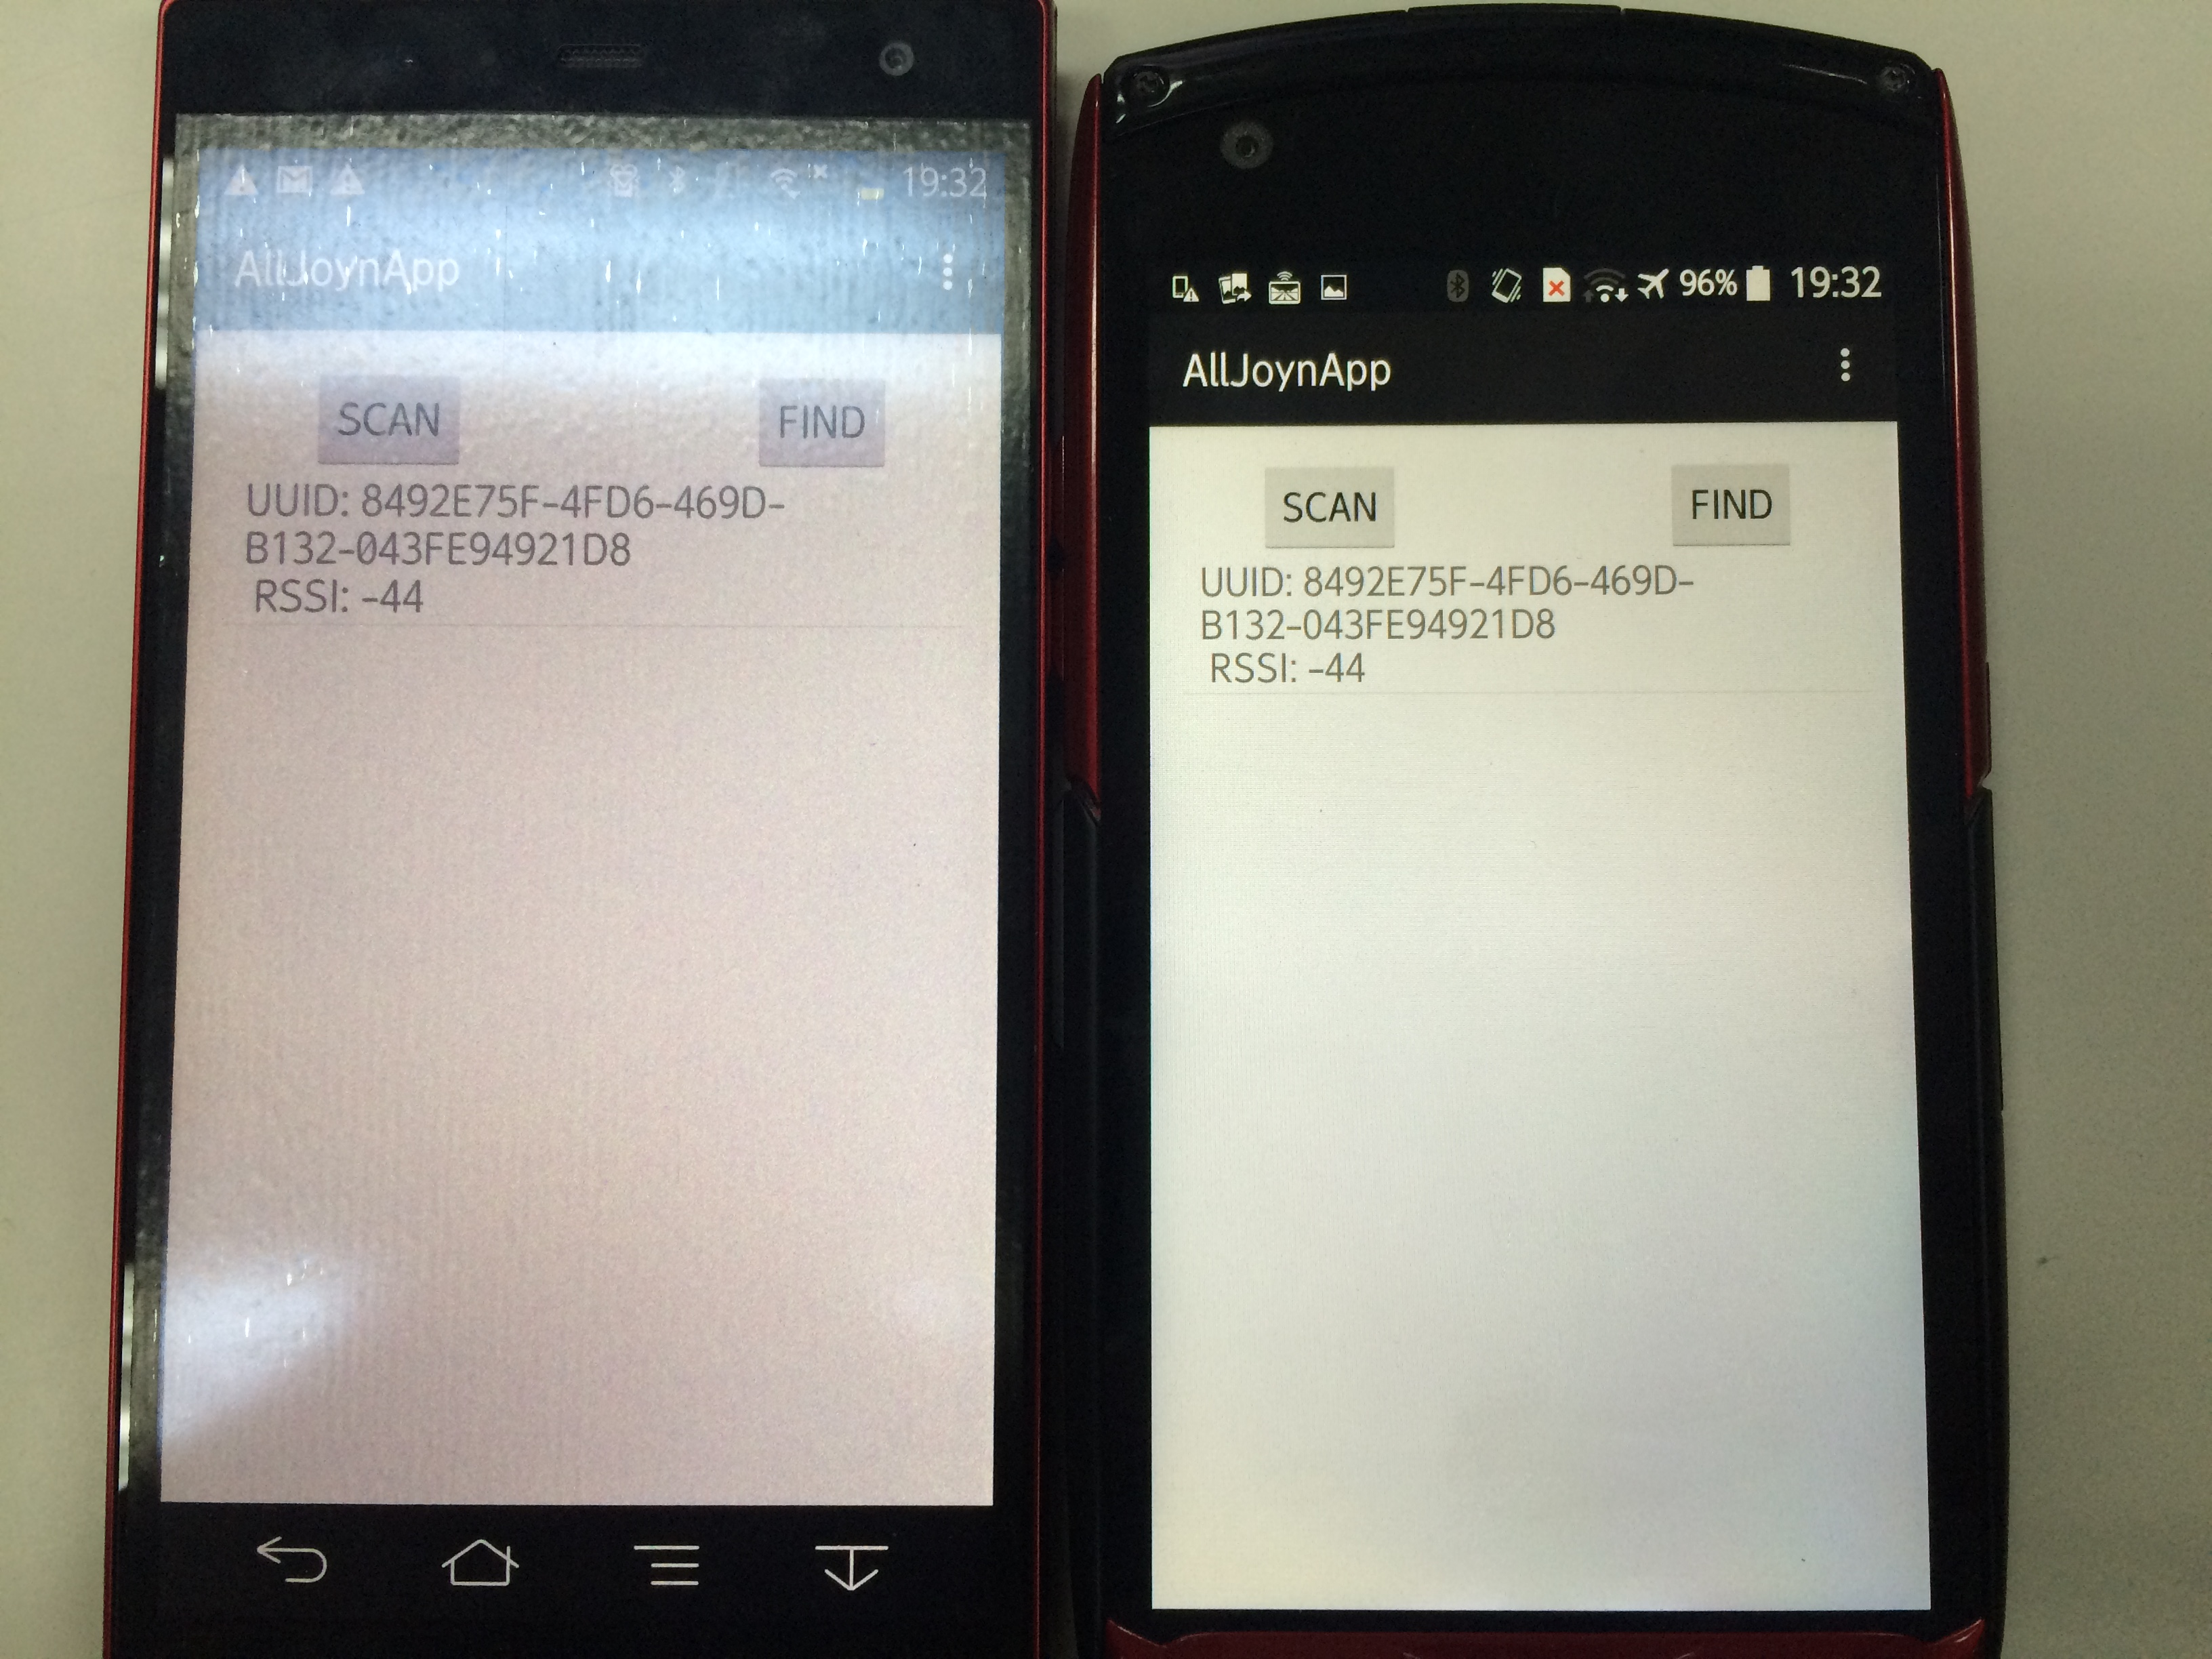
\includegraphics[width=7cm]{fig/ins_1.jpg}
    \caption{項目1}
  \end{figure}


  \newpage
  
\item 項目2 \\
  項目2の検証は項目1の手順に以下の手順を加える.
  \begin{enumerate}
  \item 発信機を停止させる.
  \item 端末AでFINDボタンを押下し,'DISCOVERY'の表示が消えたことを確認し,SCANボタンを押下する.
  \end{enumerate}

  端末A及びBの画面上に'iBeacon not found'と表示され,iBeaconの離脱を検知し,他端末に通知することができた.

  \begin{figure}[htbp]
    \centering
    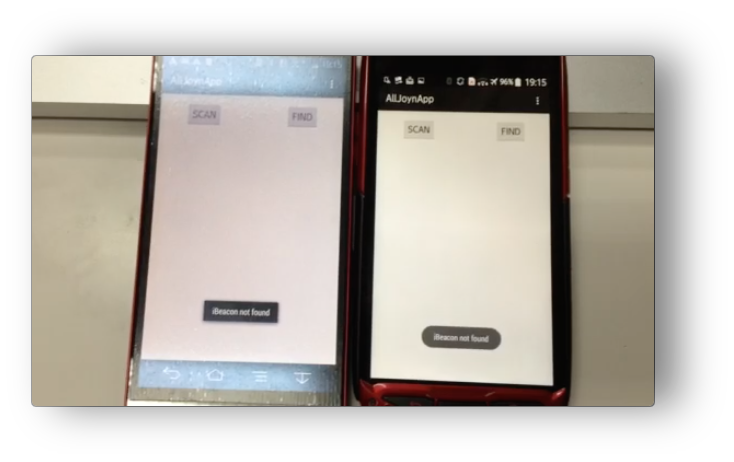
\includegraphics[width=10cm]{fig/ins_2.png}
    \caption{項目2}
  \end{figure}


\item 項目3 \\
  項目3の検証は項目1の手順に以下の手順を加える.
  \begin{enumerate}
  \item 発信機3台起動させる.
  \item 端末AでFINDボタンを押下し,'DISCOVERY'の表示が消えたことを確認し,SCANボタンを押下する.
  \end{enumerate}

  端末A及びBの画面上にiBeacon三台分のビーコン情報が表示された.
  \begin{figure}[htbp]
    \centering
    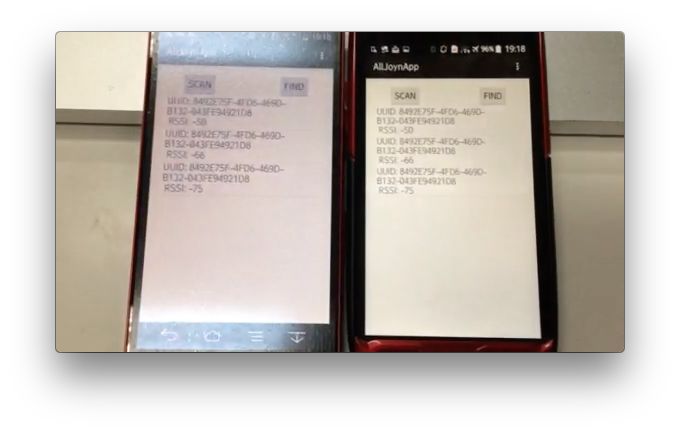
\includegraphics[width=10cm]{fig/ins_3.png}
    \caption{項目3}
  \end{figure}

\end{itemize}


\section{考察}
今回の設計・実装で,Android端末でiBeaconを検知し,ビーコン情報を他端末に送信し,ビーコン情報を共有することができた.
機材の関係上,端末二台,iBeacon発信機三台までしか検証できなかったが,検証の結果より,一般家庭や小規模の介護施設などでの見守りで使用できることが示された.
また,アクセスポイントを経由して通信を行っているので同一アクセスポイント内なら距離を選ばず通信することができるため,同一施設の異なる部屋や異なる階にいる端末とも情報共有が可能となる.

問題点としては,FINDボタンを押下してSCANボタンを押下するまで自身のAllJoynServiceを停止しているため,その間はビーコン情報の受信が出来なくなってしまうという点が挙げられる.
また,今回の実装は端末が同一アクセスポイント内にあるという想定で行ったため,屋外での見守りには対応していない.
そのため,現状では見守り可能な環境が限定されている.

他にも,「検知出来なくなったiBeaconはどれか」といった表示をしていないため,現状では大規模の見守りには不向きであるといえる.
